%%%%%%%%%%%%%%%%%%%%%%%%%%%%%%%%%%%%%%%%%%%%%%%%%%%%%%%%%%%%%%%%%%%%%%%%%%%%%%%%
%2345678901234567890123456789012345678901234567890123456789012345678901234567890
%        1         2         3         4         5         6         7         8

%\documentclass[final,letterpaper, 10 pt, conference]{ieeeconf}  % Comment this line out if you need a4paper

\documentclass[10pt, conference, compsocconf]{IEEEtran}
%\documentclass[a4paper, 10pt, conference]{ieeeconf}      % Use this line for a4 paper

%\IEEEoverridecommandlockouts                              % This command is only needed if
% you want to use the \thanks command

\newcommand{\eu}{\textrm{e}}
\newcommand{\figref}[1]{Fig.~\ref{fig:#1}}
%\overrideIEEEmargins
\usepackage[obeyFinal]{todonotes}
\RequirePackage{graphicx}
\usepackage{subfigure}
\usepackage{bm}
%\usepackage{subequation}
\graphicspath{ {Figs/} }
\usepackage{url}
%\usepackage[tight,footnotesize]{subfigure}
\usepackage{fainekos-macros}
\newcommand{\sAccu}{\epsilon}
\newcommand{\sDelay}{\delta}
\newcommand{\de}{(\sDelay,\sAccu)}
\newcommand{\dek}[1]{(\sDelay_{#1},\sAccu_{#1})}
\newcommand{\hWc}{\widehat{\Wc}}
\newcommand{\sDelayV}{\underline{\sDelay}}
\newcommand{\sAccuV}{\underline{\sAccu}}
\newcommand{\ESet}{\mathcal{E}}
%\newcommand{\bm}{\hat{B}}
\newcommand{\MPCProb}[1]{\mathbb{P_{#1}}}
\newcommand{\RAMPCProb}[2]{\mathbb{P}_{#1}(\hat{\stPt}_{#2},\sDelay_{#2},\sAccu_{#2},\inpPt_{#2 -1})}
\global\long\def\ZSet{\Zc}
\global\long\def\Cc{\mathcal{C}}
\global\long\def\Nom#1{\overline{#1}}
\newcommand{\bla}[1]{\overbar{#1}}
\newcommand{\bli}[1]{\overline{BLI #1}}

\usepackage{array}
\usepackage{url}


% See the \addtolength command later in the file to balance the column lengths
% on the last page of the document
\usepackage{amsmath} % assumes amsmath package installed
\usepackage{amssymb}  % assumes amsmath package installed
\renewcommand{\thefigure}{\arabic{figure}}
\title{\LARGE \bf
	Poster Abstract: Hardware optimizations for anytime perception and control
}


\author{\IEEEauthorblockN{Nischal K.N.$^1$, Paritosh Kelkar$^1$, Dhruva Kumar$^1$, Yash Vardhan Pant$^1$, \\
Houssam Abbas$^1$, Joseph Devietti$^2$, Rahul Mangharam$^1$}
\IEEEauthorblockA{$^1$The Department of Electrical and Systems Engineering, \\
$^2$ The Department of Computer and Information Sciences
University of Pennsylvania, \\
Philadelphia, U.S.A\\}
%{nischal,paritosh,dhruvak,yashpant,habbas,rahulm\}@seas.upenn.edu
%yashpant@seas.upenn.edu, \\habbas@seas.upenn.edu, rahulm@seas.upenn.edu}
%\and
%\IEEEauthorblockN{Joseph Devietti}
%\IEEEauthorblockA{The Department of Computer\\  and Information Sciences, \\
%University of Pennsylvania, \\
%Philadelphia, U.S.A\\
%devietti@cis.upenn.edu}
}







%\author{ Nischal K.N., Paritosh Kelkar, Dhruva Kumar, Yash Vardhan Pant, Houssam Abbas\\
%	Joseph Devietti, Rahul Mangharam% <-this % stops a space
%	\thanks{*This work was supported by STARnet a Semiconductor Research
%		Corporation program sponsored by MARCO and DARPA, NSF MRI-0923518 and the US Department of Transportation University Transportation Center Program}% <-this % stops a space
%	\thanks{The Departments of Electrical and Systems Engineering and Computer and Information Sciences, University of Pennsylvania, Philadelphia, U.S.A.
		{\small
%			 \{nischal,paritosh,dhruvak,yashpant,habbas,rahulm\}@seas.upenn.edu, %devietti@cis.upenn.edu}}%
%}


\begin{document}
	
\maketitle
\thispagestyle{empty}
\pagestyle{empty}

In recent years, the development of autonomous vehicles (AVs) has become a major component of the roadmaps of most large automotive manufacturers. 
The perception and control software of these systems have stringent real-time requirements that have to be met for their safe and correct operation.
The uncertain environment in which the AV operates and its complete reliance on sensor data leads to over-engineering, where the system is designed to operate as if the worst-case conditions always hold.
This leads to unnecessarily high power consumption, especially when we consider the large amount of data produced and processed in an AV (from on-board cameras, LIDAR, radars, ultrasonic sensors, high precision GPS, etc). 

In this poster, we present early results of our experiments on a $1/10^{th}$ scale autonomous car. 
The objective of the experiments is to obtain more energy-efficient computations for the perception and estimation algorithms used in autonomous systems by exploiting hardware-level knobs. 
These knobs allow us to leverage a trade-off between computation time, power consumption and output quality of the perception and estimation algorithms. 
In this case, we use a Vanishing Point algorithm to navigate a corridor. 
Vanishing Point is decomposed into three sequential components, and we study how its runtime and power consumption are affected by whether each component is run on a GPU or CPU, and the frequency at which it is executed.
Results highlight CPU/GPU allocation and execution frequencies which achieve better throughput or better power.

Our general method is concerned with how these time/power/quality trade-offs affect control performance. 
We seek to design controllers that can leverage this trade-off to maintain control performance at a lower power cost, or react to a very dynamic driving situation intelligently by obtaining lower quality but more timely estimates of the system's state.   
In the case of the Vanishing Point algorithm, for example, the controller decides at run-time, and for each time step, whether to schedule each of the algorithms's components on the CPU or GPU and at what frequency, to achieve control performance at minimal power. The possible set of operating points and their effect on the update rate and power consumption for the vanishing point algorithm are shown in Figs. \ref{fig:sfda},\ref{fig:sfda_pow}. For each of the three tasks we consider, C (G) represents execution on the CPU (GPU). We can see that a single operating point does not always achieve best overall performance for both update rate and power consumption.
%Ongoing work is focussed on using this profile at run-time and closing the loop with feedback control while selecting operating points for vanishing point on the fly.

\begin{figure}[htbp]
	\centering
	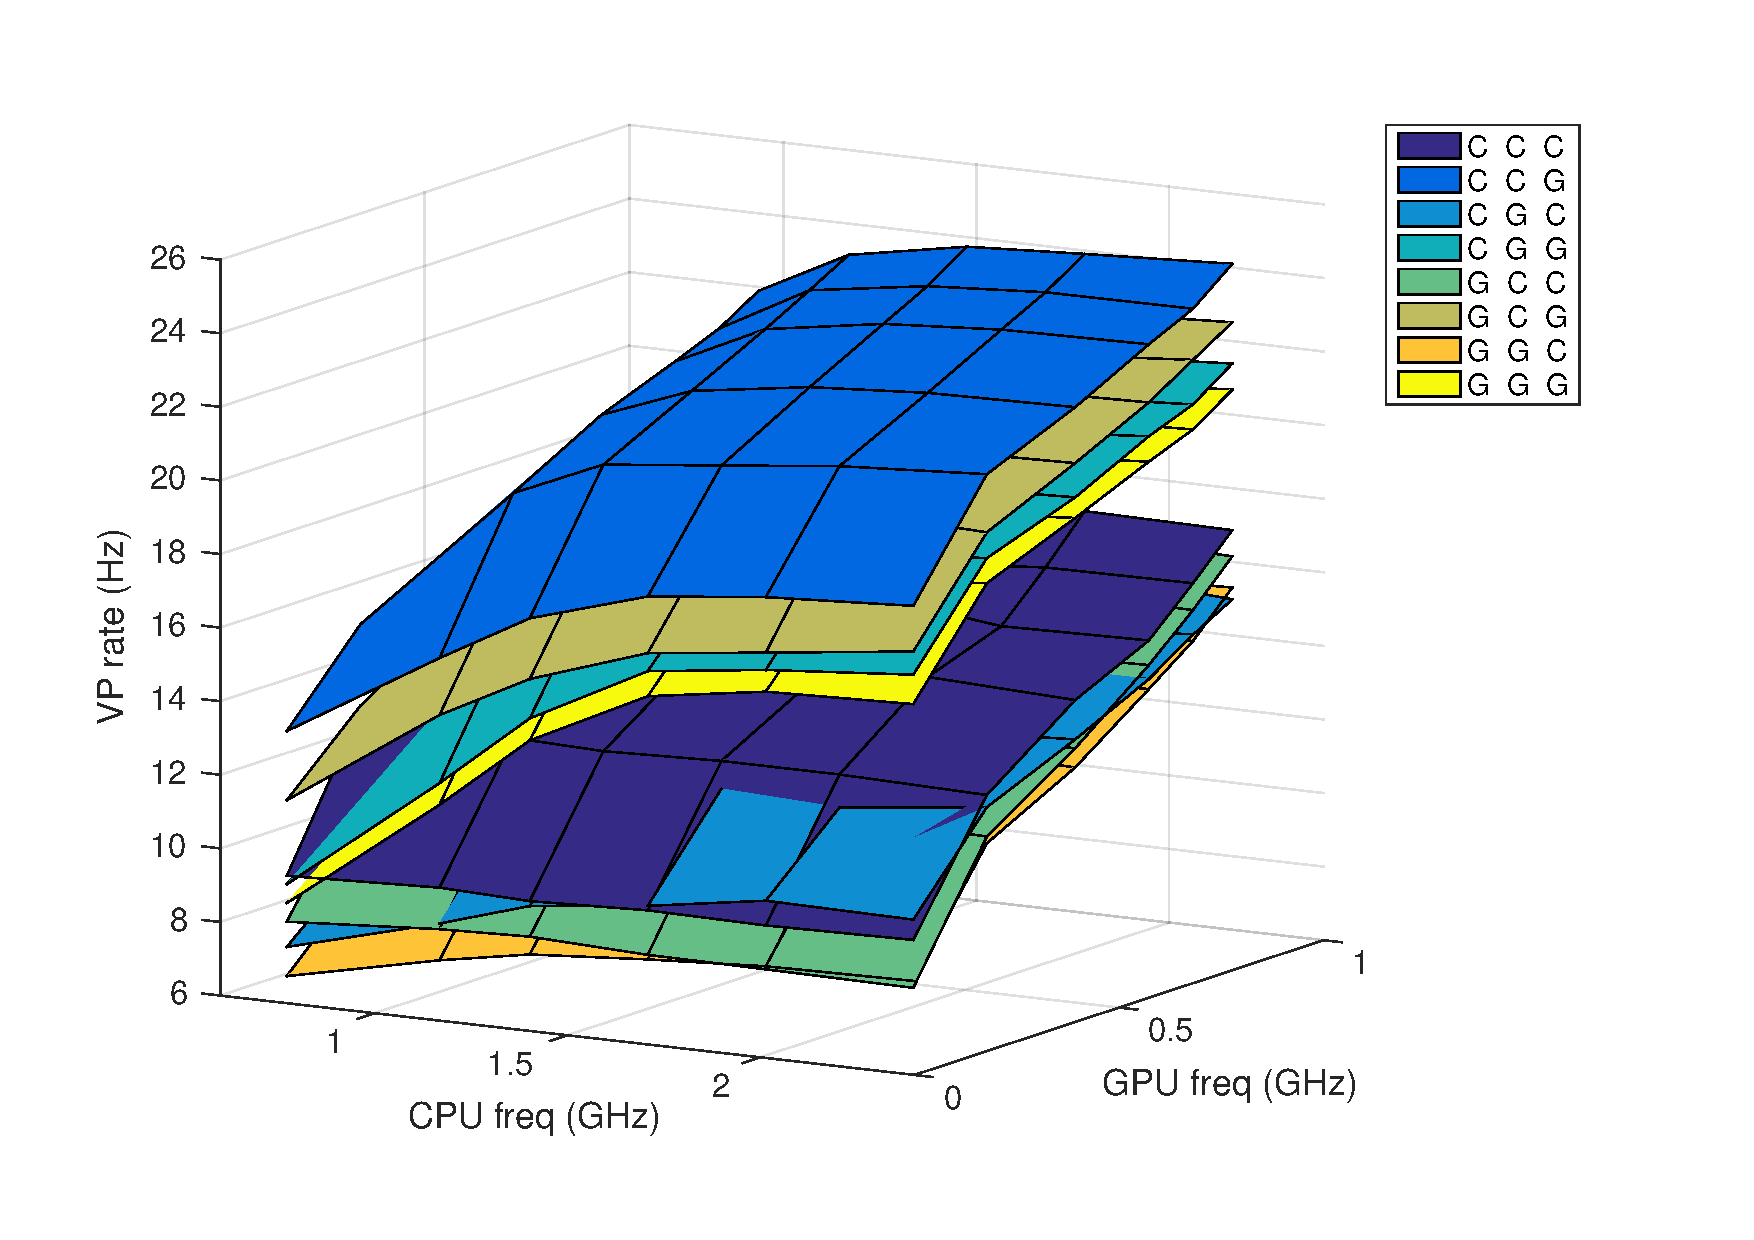
\includegraphics[width=0.46\textwidth]{Data/figs/surf_Rate.pdf}
	\caption{Control update rate for different CPU-GPU assignments at varying frequencies (color in online version).}
	\label{fig:sfda}%same freq diff assignment}
\end{figure}
	%\bibliographystyle{IEEEtran}%abbrv}
	%\bibliography{IEEEabrv,rtss2015,cdc14,anytime_ref,rtss_wip_ref}


\begin{figure}[htbp]
	\centering
	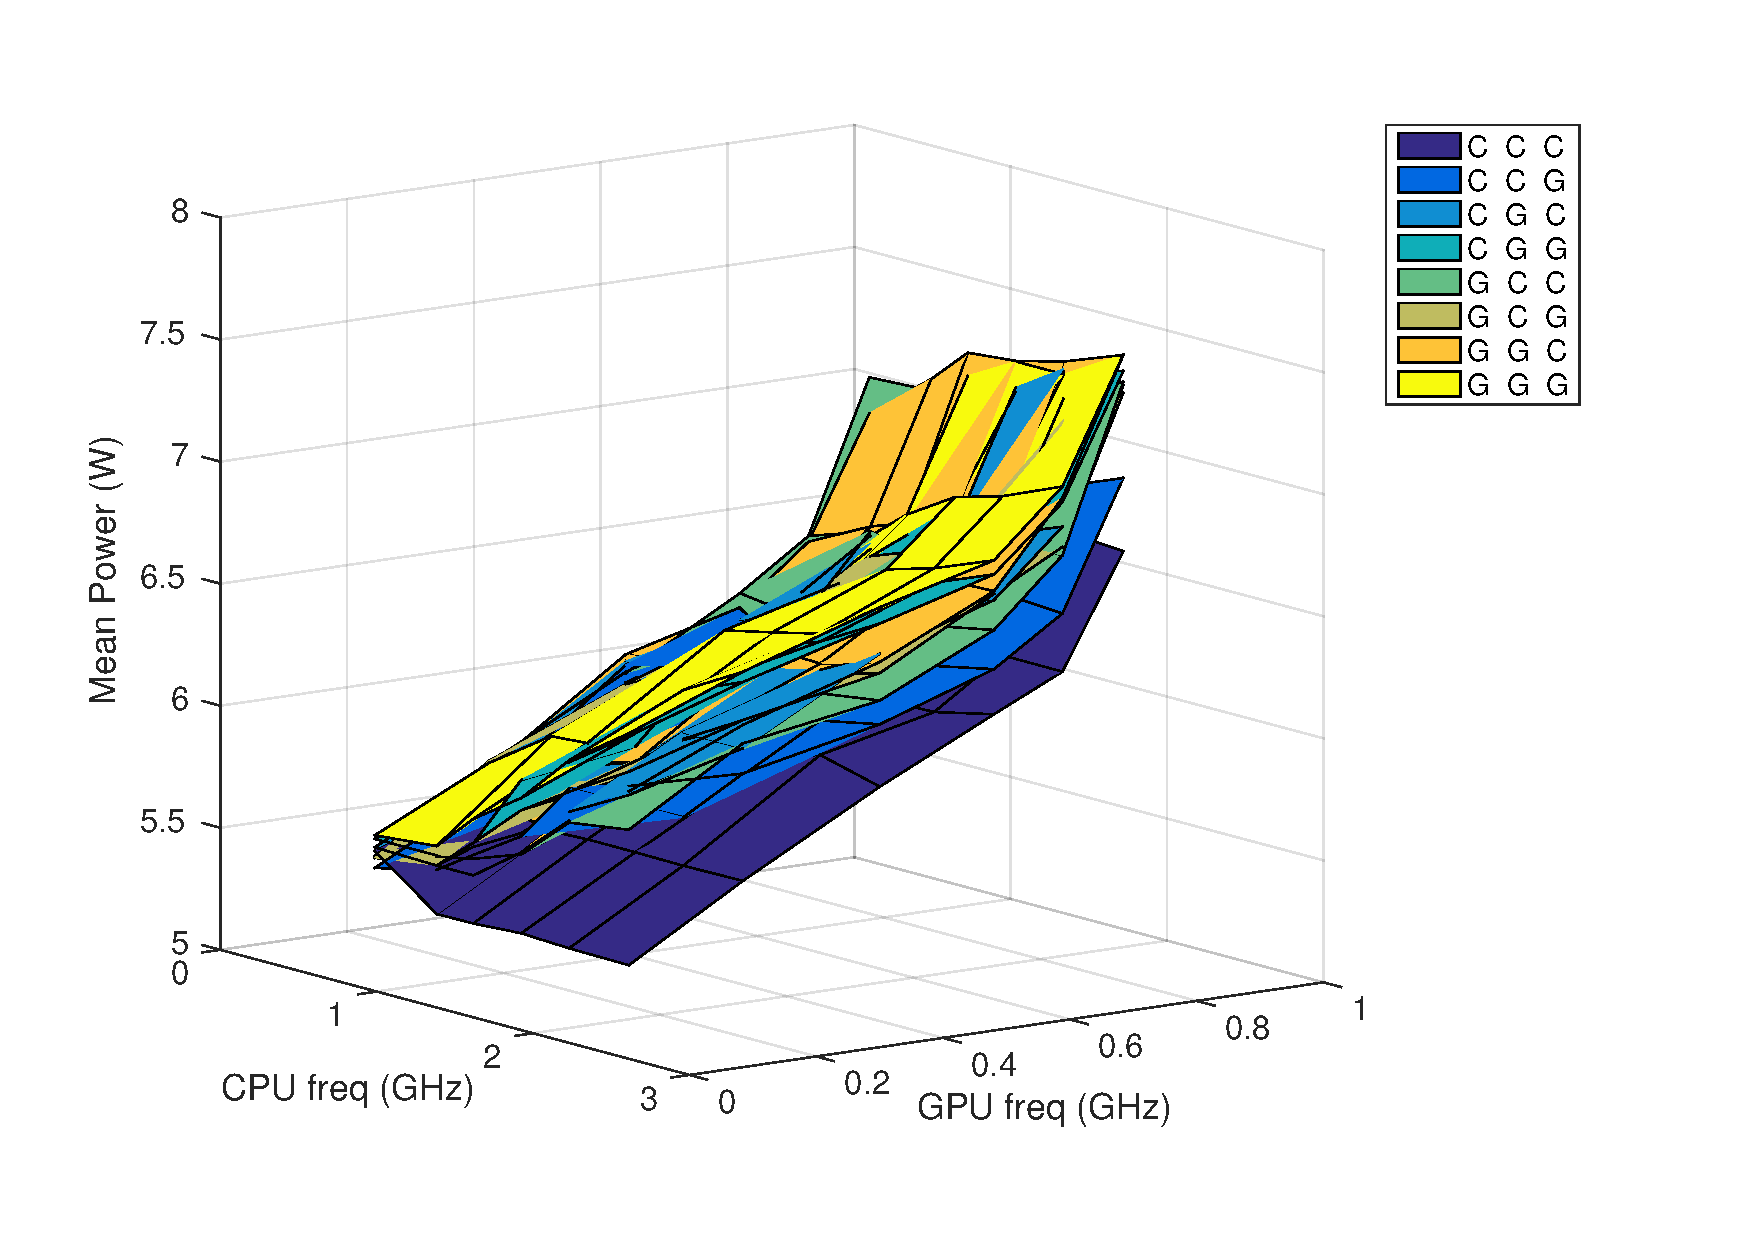
\includegraphics[width=0.46\textwidth]{Data/figs/surf_Power.pdf}
	\caption{Mean power consumed by the vanishing point algorithm (running on the Nvidia Jetson) for different CPU-GPU assignments at varying frequencies. (Color in online version).}
	\label{fig:sfda_pow}%same freq diff assignment}
\end{figure}



\section*{Acknowledgments}
This work was supported by STARnet a Semiconductor Research Corporation program sponsored by MARCO and DARPA, NSF MRI-0923518 and the US Department of Transportation University Transportation Center Program. 
	
\end{document}

